\section{Introduction}\raggedbottom

\subsection{Electrocardiographic Data}
Electrocardiographic data is obtained by placing electrodes on different parts of the body, mainly around the heart, which measure the electrical changes in voltage over time, produced by the heart muscle \autocite{ElectrocardiographyWikipedia-2021-01-14}. Multiple electrodes are placed to get a better overview over the heart state, since other muscles will add noise under non ideal conditions. A high recording frequency of 257-10000hz and a recording length of 10 seconds up to 30 minutes\footnote{attributes of ECG data reported from \ref{itm:itemize-datas}} or even days (long time ECG used in hospitals) are desirable to not miss important information that could reveal an infarction and other muscular heart diseases.
 
We obtain sequential data that can be classified like other time-series, however since each individual electrode produces its own signal there is more than one data channel to analyze concurrently, which increases the difficulty to find a generalizing computer system. For example the conventional "12-lead ECG" uses 10 differently placed electrodes resulting in 12 different channels together with the two additional ones added by averaging \autocite{12LeadECGPlacementGuidewithIllustrations-2021-09-28}. Accounting for the high frequency and length this would sum up to $\mathbf{data points}=\mathbf{seconds}*\mathbf{frequency}*\mathbf{channels}=10\mathbf{s}*1000\mathbf{hz}*12=120000$ data points for short recordings or $120\mathbf{s}*1000\mathbf{hz}*12=1440000$ data points for longer recordings, per patient (assuming a frequency of 1000hz). The varying lengths and much information make correct prediction challenging. For comparison, the widely used ImageNet \autocite{ImageNet-2021-01-14} counts on average $469\times387$ pixels\autocite{stack-imagenet}, which is equal to $469*387*3=544509$ data points. Additionally the recordings can contain more than one \enquote{true} label which makes correct classification even more difficult. Like in many medical fields, one big hurdle in training a fully automated system is the inaccessible correctly labeled data. The biggest reason for the data scarcity is that only trained professionals/doctors are able to successfully diagnose patients, while also requiring long periods of time to do so.  

Nevertheless we found a few dataset sources that are openly available online:
\begin{itemize}
	\item[PTB] A dataset provided by the Physikalisch-Technische Bundesanstalt (PTB) containing 549 records with 9 diagnostic class labels. \autocite{ptb}
	\item[PTB-XL] A dataset provided by the Physikalisch-Technische Bundesanstalt (PTB) containining 21837 records with 52 diagnostic class labels (5 superclasses, split into 52 unique scp codes).\autocite{ptbxl}
	\item[Georgia] \enquote{Georgia} dataset which is hosted on \url{Kaggle.com} \autocite{Georgia12LeadECGChallengeDatabaseKaggle-2021-03-15}
	\item[China] A dataset provided during a chinese classification challenge and made openly available.
	\item[Nature] A 12-lead electrocardiogram database for arrhythmia research covering more than 10,000 patients. \autocite{Zheng2020}
	\label{itm:itemize-datas}
\end{itemize}
Most of the above datasets and more are also used in a recent ECG classification challenge from 2020 \autocite{PerezAlday2021} hosted by physionet.org \autocite{physionet}. Since the original datasets have incompatible labels (e.g. the same classes are mapped to different terms) we use the available challenge data because the labels across all datasets were already mapped to unique SNOMED CT codes \autocite{SNOMEDCTClasses}. The \enquote{Nature} data labels, which are not part of the challenge data, had to be dropped since they were incompatible to the other datasets, thus this data will be only used in pretraining for models that require it.

The data has 12 channels and one or more \enquote{true} labels per sample. However there is no hint on to where the label is found in the sequential data. See \autoref{fig:ECGBasic} for an example ECG recording.
\begin{figure}[H]
	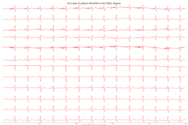
\includegraphics[width=\textwidth]{bilder/ecg-example0.png}
	\caption{A single patients ECG with 500hz recording frequency. The classes \textit{EKG: T wave abnormal} and \textit{sinus rhythm} can both be found somewhere in the data.}
	\label{fig:ECGBasic}
\end{figure}
To better understand the data we count class occurrences over all datasets, with their respective SNOMED Code and the index number used in our implementation \autoref{table:ClassCounts}. Readily identifiable is that not every class is present in all datasets and that some classes are very rare in comparison to others. Additionally some classes are closely related or even superclasses of others but are not consistently stated as true even though the subclass is true (see Bundle Branch Block vs. left/right Bundle Branch Block or Ventricular Hypertrophy vs. left/right Ventricular Hypertrophy). Since some class distinctions might be intentional, we did not apply any changes to the labels, but want to point out the possible classification difficulty increase due to the label inconsistencies. 

\begin{figure}[H]
	\caption{All SNOMED Codes with their respective name and count in the datasets.}
	\resizebox{!}{0.8\textwidth}{
		\begin{tabular}{lllrrrr}
{} & {} & {} & {ptbxl} & {georgia} & {cpsc} & {cpsc2} \\
{Index} & {Class Snomed Code} & {Class Term} & {} & {} & {} & {} \\
0 & 10370003 & Rhythm from artificial pacing (298) & {\cellcolor[HTML]{2E8B57}} \color[HTML]{F1F1F1} 295 & {\cellcolor[HTML]{EBF3ED}} \color[HTML]{000000} 0 & {\cellcolor[HTML]{EBF3ED}} \color[HTML]{000000} 0 & {\cellcolor[HTML]{E9F2EC}} \color[HTML]{000000} 3 \\
1 & 11157007 & Ventricular bigeminy (89) & {\cellcolor[HTML]{2E8B57}} \color[HTML]{F1F1F1} 82 & {\cellcolor[HTML]{E7F0EA}} \color[HTML]{000000} 2 & {\cellcolor[HTML]{EBF3ED}} \color[HTML]{000000} 0 & {\cellcolor[HTML]{E0ECE4}} \color[HTML]{000000} 5 \\
2 & 111975006 & Prolonged QT interval (1493) & {\cellcolor[HTML]{DBEAE0}} \color[HTML]{000000} 118 & {\cellcolor[HTML]{2E8B57}} \color[HTML]{F1F1F1} 1372 & {\cellcolor[HTML]{EBF3ED}} \color[HTML]{000000} 0 & {\cellcolor[HTML]{EBF3ED}} \color[HTML]{000000} 3 \\
3 & 164861001 & EKG myocardial ischemia (2556) & {\cellcolor[HTML]{2E8B57}} \color[HTML]{F1F1F1} 2175 & {\cellcolor[HTML]{EBF3ED}} \color[HTML]{000000} 0 & {\cellcolor[HTML]{EBF3ED}} \color[HTML]{000000} 0 & {\cellcolor[HTML]{CAE1D3}} \color[HTML]{000000} 381 \\
4 & 164865005 & EKG: myocardial infarction (5640) & {\cellcolor[HTML]{2E8B57}} \color[HTML]{F1F1F1} 5261 & {\cellcolor[HTML]{EBF3ED}} \color[HTML]{000000} 7 & {\cellcolor[HTML]{EBF3ED}} \color[HTML]{000000} 0 & {\cellcolor[HTML]{DEEBE3}} \color[HTML]{000000} 372 \\
5 & 164867002 & EKG: old myocardial infarction (1160) & {\cellcolor[HTML]{EBF3ED}} \color[HTML]{000000} 0 & {\cellcolor[HTML]{EBF3ED}} \color[HTML]{000000} 0 & {\cellcolor[HTML]{EBF3ED}} \color[HTML]{000000} 0 & {\cellcolor[HTML]{2E8B57}} \color[HTML]{F1F1F1} 1160 \\
6 & 164873001 & EKG:left ventricle hypertrophy (3735) & {\cellcolor[HTML]{2E8B57}} \color[HTML]{F1F1F1} 2359 & {\cellcolor[HTML]{88BD9F}} \color[HTML]{000000} 1226 & {\cellcolor[HTML]{EBF3ED}} \color[HTML]{000000} 0 & {\cellcolor[HTML]{DFECE4}} \color[HTML]{000000} 150 \\
7 & 164884008 & ECG: ventricular ectopics (1894) & {\cellcolor[HTML]{2E8B57}} \color[HTML]{F1F1F1} 1154 & {\cellcolor[HTML]{E4EFE8}} \color[HTML]{000000} 41 & {\cellcolor[HTML]{78B492}} \color[HTML]{F1F1F1} 699 & {\cellcolor[HTML]{EBF3ED}} \color[HTML]{000000} 0 \\
8 & 164889003 & ECG: atrial fibrillation (3441) & {\cellcolor[HTML]{2E8B57}} \color[HTML]{F1F1F1} 1514 & {\cellcolor[HTML]{B2D3C0}} \color[HTML]{000000} 561 & {\cellcolor[HTML]{57A177}} \color[HTML]{F1F1F1} 1219 & {\cellcolor[HTML]{EBF3ED}} \color[HTML]{000000} 147 \\
9 & 164890007 & EKG: atrial flutter (303) & {\cellcolor[HTML]{A0CAB2}} \color[HTML]{000000} 73 & {\cellcolor[HTML]{2E8B57}} \color[HTML]{F1F1F1} 185 & {\cellcolor[HTML]{EBF3ED}} \color[HTML]{000000} 0 & {\cellcolor[HTML]{BDD9C9}} \color[HTML]{000000} 45 \\
10 & 164909002 & EKG: left bundle branch block (1038) & {\cellcolor[HTML]{2E8B57}} \color[HTML]{F1F1F1} 536 & {\cellcolor[HTML]{A2CBB3}} \color[HTML]{000000} 229 & {\cellcolor[HTML]{A0CAB2}} \color[HTML]{000000} 235 & {\cellcolor[HTML]{EBF3ED}} \color[HTML]{000000} 38 \\
11 & 164917005 & EKG: Q wave abnormal (1010) & {\cellcolor[HTML]{2E8B57}} \color[HTML]{F1F1F1} 548 & {\cellcolor[HTML]{4C9B6F}} \color[HTML]{F1F1F1} 461 & {\cellcolor[HTML]{EBF3ED}} \color[HTML]{000000} 0 & {\cellcolor[HTML]{EBF3ED}} \color[HTML]{000000} 1 \\
12 & 164930006 & ECG: ST interval abnormal (1453) & {\cellcolor[HTML]{EBF3ED}} \color[HTML]{000000} 0 & {\cellcolor[HTML]{2E8B57}} \color[HTML]{F1F1F1} 979 & {\cellcolor[HTML]{EBF3ED}} \color[HTML]{000000} 0 & {\cellcolor[HTML]{90C1A5}} \color[HTML]{000000} 474 \\
13 & 164931005 & ST elevation (444) & {\cellcolor[HTML]{EBF3ED}} \color[HTML]{000000} 28 & {\cellcolor[HTML]{83BA9B}} \color[HTML]{000000} 133 & {\cellcolor[HTML]{2E8B57}} \color[HTML]{F1F1F1} 220 & {\cellcolor[HTML]{C9E0D2}} \color[HTML]{000000} 63 \\
14 & 164934002 & EKG: T wave abnormal (4651) & {\cellcolor[HTML]{2E8B57}} \color[HTML]{F1F1F1} 2345 & {\cellcolor[HTML]{328D5B}} \color[HTML]{F1F1F1} 2284 & {\cellcolor[HTML]{EBF3ED}} \color[HTML]{000000} 0 & {\cellcolor[HTML]{E9F2EC}} \color[HTML]{000000} 22 \\
15 & 164947007 & Prolonged PR interval (340) & {\cellcolor[HTML]{2E8B57}} \color[HTML]{F1F1F1} 340 & {\cellcolor[HTML]{EBF3ED}} \color[HTML]{000000} 0 & {\cellcolor[HTML]{EBF3ED}} \color[HTML]{000000} 0 & {\cellcolor[HTML]{EBF3ED}} \color[HTML]{000000} 0 \\
16 & 164951009 & EKG: QRS complex abnormal (3389) & {\cellcolor[HTML]{2E8B57}} \color[HTML]{F1F1F1} 3389 & {\cellcolor[HTML]{EBF3ED}} \color[HTML]{000000} 0 & {\cellcolor[HTML]{EBF3ED}} \color[HTML]{000000} 0 & {\cellcolor[HTML]{EBF3ED}} \color[HTML]{000000} 0 \\
17 & 17338001 & Ventricular premature beats (359) & {\cellcolor[HTML]{EBF3ED}} \color[HTML]{000000} 0 & {\cellcolor[HTML]{2E8B57}} \color[HTML]{F1F1F1} 351 & {\cellcolor[HTML]{EBF3ED}} \color[HTML]{000000} 0 & {\cellcolor[HTML]{E7F1EA}} \color[HTML]{000000} 8 \\
18 & 195042002 & Second degree atrioventricular block (58) & {\cellcolor[HTML]{78B492}} \color[HTML]{F1F1F1} 14 & {\cellcolor[HTML]{2E8B57}} \color[HTML]{F1F1F1} 23 & {\cellcolor[HTML]{EBF3ED}} \color[HTML]{000000} 0 & {\cellcolor[HTML]{3E9464}} \color[HTML]{F1F1F1} 21 \\
19 & 195080001 & Atrial fibrillation and flutter (39) & {\cellcolor[HTML]{EBF3ED}} \color[HTML]{000000} 0 & {\cellcolor[HTML]{E1EDE6}} \color[HTML]{000000} 2 & {\cellcolor[HTML]{EBF3ED}} \color[HTML]{000000} 0 & {\cellcolor[HTML]{2E8B57}} \color[HTML]{F1F1F1} 37 \\
20 & 195126007 & Atrial hypertrophy (61) & {\cellcolor[HTML]{EBF3ED}} \color[HTML]{000000} 0 & {\cellcolor[HTML]{2E8B57}} \color[HTML]{F1F1F1} 59 & {\cellcolor[HTML]{EBF3ED}} \color[HTML]{000000} 0 & {\cellcolor[HTML]{E5EFE9}} \color[HTML]{000000} 2 \\
21 & 233917008 & Atrioventricular block (77) & {\cellcolor[HTML]{EBF3ED}} \color[HTML]{000000} 0 & {\cellcolor[HTML]{2E8B57}} \color[HTML]{F1F1F1} 74 & {\cellcolor[HTML]{EBF3ED}} \color[HTML]{000000} 0 & {\cellcolor[HTML]{E4EEE7}} \color[HTML]{000000} 3 \\
22 & 251120003 & Incomplete left bundle branch block (201) & {\cellcolor[HTML]{3B9262}} \color[HTML]{F1F1F1} 77 & {\cellcolor[HTML]{2E8B57}} \color[HTML]{F1F1F1} 83 & {\cellcolor[HTML]{EBF3ED}} \color[HTML]{000000} 0 & {\cellcolor[HTML]{8EBFA3}} \color[HTML]{000000} 41 \\
23 & 251146004 & Low QRS voltages (552) & {\cellcolor[HTML]{8EC0A4}} \color[HTML]{000000} 182 & {\cellcolor[HTML]{2E8B57}} \color[HTML]{F1F1F1} 370 & {\cellcolor[HTML]{EBF3ED}} \color[HTML]{000000} 0 & {\cellcolor[HTML]{EBF3ED}} \color[HTML]{000000} 0 \\
24 & 251180001 & Ventricular trigeminy (24) & {\cellcolor[HTML]{2E8B57}} \color[HTML]{F1F1F1} 20 & {\cellcolor[HTML]{E2EEE6}} \color[HTML]{000000} 1 & {\cellcolor[HTML]{EBF3ED}} \color[HTML]{000000} 0 & {\cellcolor[HTML]{CFE3D7}} \color[HTML]{000000} 3 \\
25 & 251200008 & Indeterminate cardiac axis (156) & {\cellcolor[HTML]{2E8B57}} \color[HTML]{F1F1F1} 156 & {\cellcolor[HTML]{EBF3ED}} \color[HTML]{000000} 0 & {\cellcolor[HTML]{EBF3ED}} \color[HTML]{000000} 0 & {\cellcolor[HTML]{EBF3ED}} \color[HTML]{000000} 0 \\
26 & 251266004 & Ventricular pacing pattern (43) & {\cellcolor[HTML]{EBF3ED}} \color[HTML]{000000} 0 & {\cellcolor[HTML]{2E8B57}} \color[HTML]{F1F1F1} 43 & {\cellcolor[HTML]{EBF3ED}} \color[HTML]{000000} 0 & {\cellcolor[HTML]{EBF3ED}} \color[HTML]{000000} 0 \\
27 & 251268003 & Atrial pacing pattern (50) & {\cellcolor[HTML]{EBF3ED}} \color[HTML]{000000} 0 & {\cellcolor[HTML]{2E8B57}} \color[HTML]{F1F1F1} 50 & {\cellcolor[HTML]{EBF3ED}} \color[HTML]{000000} 0 & {\cellcolor[HTML]{EBF3ED}} \color[HTML]{000000} 0 \\
28 & 253352002 & Left atrial abnormality (70) & {\cellcolor[HTML]{EBF3ED}} \color[HTML]{000000} 0 & {\cellcolor[HTML]{2E8B57}} \color[HTML]{F1F1F1} 70 & {\cellcolor[HTML]{EBF3ED}} \color[HTML]{000000} 0 & {\cellcolor[HTML]{EBF3ED}} \color[HTML]{000000} 0 \\
29 & 266249003 & Ventricular hypertrophy (105) & {\cellcolor[HTML]{9AC6AD}} \color[HTML]{000000} 30 & {\cellcolor[HTML]{2E8B57}} \color[HTML]{F1F1F1} 70 & {\cellcolor[HTML]{EBF3ED}} \color[HTML]{000000} 0 & {\cellcolor[HTML]{DEEBE3}} \color[HTML]{000000} 5 \\
30 & 270492004 & First degree atrioventricular block (2385) & {\cellcolor[HTML]{2E8B57}} \color[HTML]{F1F1F1} 797 & {\cellcolor[HTML]{37905E}} \color[HTML]{F1F1F1} 764 & {\cellcolor[HTML]{439667}} \color[HTML]{F1F1F1} 721 & {\cellcolor[HTML]{EBF3ED}} \color[HTML]{000000} 103 \\
31 & 27885002 & Complete atrioventricular block (46) & {\cellcolor[HTML]{61A780}} \color[HTML]{F1F1F1} 16 & {\cellcolor[HTML]{A6CDB6}} \color[HTML]{000000} 8 & {\cellcolor[HTML]{EBF3ED}} \color[HTML]{000000} 0 & {\cellcolor[HTML]{2E8B57}} \color[HTML]{F1F1F1} 22 \\
32 & 284470004 & Premature atrial contraction (1722) & {\cellcolor[HTML]{7DB696}} \color[HTML]{F1F1F1} 398 & {\cellcolor[HTML]{2E8B57}} \color[HTML]{F1F1F1} 635 & {\cellcolor[HTML]{348E5C}} \color[HTML]{F1F1F1} 616 & {\cellcolor[HTML]{EBF3ED}} \color[HTML]{000000} 73 \\
33 & 39732003 & Left axis deviation (6080) & {\cellcolor[HTML]{2E8B57}} \color[HTML]{F1F1F1} 5146 & {\cellcolor[HTML]{C9E0D2}} \color[HTML]{000000} 934 & {\cellcolor[HTML]{EBF3ED}} \color[HTML]{000000} 0 & {\cellcolor[HTML]{EBF3ED}} \color[HTML]{000000} 0 \\
34 & 413844008 & Chronic myocardial ischemia (160) & {\cellcolor[HTML]{EBF3ED}} \color[HTML]{000000} 0 & {\cellcolor[HTML]{EBF3ED}} \color[HTML]{000000} 0 & {\cellcolor[HTML]{EBF3ED}} \color[HTML]{000000} 0 & {\cellcolor[HTML]{2E8B57}} \color[HTML]{F1F1F1} 160 \\
35 & 425419005 & EKG: inferior ischemia (660) & {\cellcolor[HTML]{8DBFA2}} \color[HTML]{000000} 219 & {\cellcolor[HTML]{2E8B57}} \color[HTML]{F1F1F1} 441 & {\cellcolor[HTML]{EBF3ED}} \color[HTML]{000000} 0 & {\cellcolor[HTML]{EBF3ED}} \color[HTML]{000000} 0 \\
36 & 425623009 & EKG: lateral ischemia (1039) & {\cellcolor[HTML]{CDE2D6}} \color[HTML]{000000} 142 & {\cellcolor[HTML]{2E8B57}} \color[HTML]{F1F1F1} 897 & {\cellcolor[HTML]{EBF3ED}} \color[HTML]{000000} 0 & {\cellcolor[HTML]{EBF3ED}} \color[HTML]{000000} 0 \\
37 & 426177001 & ECG: sinus bradycardia (2351) & {\cellcolor[HTML]{A3CBB4}} \color[HTML]{000000} 637 & {\cellcolor[HTML]{2E8B57}} \color[HTML]{F1F1F1} 1670 & {\cellcolor[HTML]{EBF3ED}} \color[HTML]{000000} 0 & {\cellcolor[HTML]{E7F0EA}} \color[HTML]{000000} 44 \\
38 & 426434006 & EKG: anterior ischemia (323) & {\cellcolor[HTML]{CDE2D6}} \color[HTML]{000000} 44 & {\cellcolor[HTML]{2E8B57}} \color[HTML]{F1F1F1} 279 & {\cellcolor[HTML]{EBF3ED}} \color[HTML]{000000} 0 & {\cellcolor[HTML]{EBF3ED}} \color[HTML]{000000} 0 \\
39 & 426627000 & ECG: bradycardia (273) & {\cellcolor[HTML]{EBF3ED}} \color[HTML]{000000} 0 & {\cellcolor[HTML]{E7F1EA}} \color[HTML]{000000} 6 & {\cellcolor[HTML]{EBF3ED}} \color[HTML]{000000} 0 & {\cellcolor[HTML]{2E8B57}} \color[HTML]{F1F1F1} 267 \\
40 & 426761007 & EKG: supraventricular tachycardia (62) & {\cellcolor[HTML]{4B9B6E}} \color[HTML]{F1F1F1} 27 & {\cellcolor[HTML]{2E8B57}} \color[HTML]{F1F1F1} 32 & {\cellcolor[HTML]{EBF3ED}} \color[HTML]{000000} 0 & {\cellcolor[HTML]{D9E9DF}} \color[HTML]{000000} 3 \\
41 & 426783006 & ECG: sinus rhythm (20760) & {\cellcolor[HTML]{2E8B57}} \color[HTML]{F1F1F1} 18090 & {\cellcolor[HTML]{D9E9DF}} \color[HTML]{000000} 1751 & {\cellcolor[HTML]{E2EEE6}} \color[HTML]{000000} 916 & {\cellcolor[HTML]{EBF3ED}} \color[HTML]{000000} 3 \\
42 & 427084000 & ECG: sinus tachycardia (2374) & {\cellcolor[HTML]{6EAE8A}} \color[HTML]{F1F1F1} 826 & {\cellcolor[HTML]{2E8B57}} \color[HTML]{F1F1F1} 1247 & {\cellcolor[HTML]{EBF3ED}} \color[HTML]{000000} 0 & {\cellcolor[HTML]{BEDAC9}} \color[HTML]{000000} 301 \\
43 & 427172004 & ECG: premature ventricular contractions (178) & {\cellcolor[HTML]{EBF3ED}} \color[HTML]{000000} 0 & {\cellcolor[HTML]{EBF3ED}} \color[HTML]{000000} 0 & {\cellcolor[HTML]{EBF3ED}} \color[HTML]{000000} 0 & {\cellcolor[HTML]{2E8B57}} \color[HTML]{F1F1F1} 178 \\
44 & 427393009 & ECG: sinus arrhythmia (1234) & {\cellcolor[HTML]{2E8B57}} \color[HTML]{F1F1F1} 772 & {\cellcolor[HTML]{7DB695}} \color[HTML]{F1F1F1} 452 & {\cellcolor[HTML]{EBF3ED}} \color[HTML]{000000} 0 & {\cellcolor[HTML]{E9F1EB}} \color[HTML]{000000} 10 \\
45 & 428417006 & Early repolarization (138) & {\cellcolor[HTML]{EBF3ED}} \color[HTML]{000000} 0 & {\cellcolor[HTML]{2E8B57}} \color[HTML]{F1F1F1} 138 & {\cellcolor[HTML]{EBF3ED}} \color[HTML]{000000} 0 & {\cellcolor[HTML]{EBF3ED}} \color[HTML]{000000} 0 \\
46 & 428750005 & Nonspecific ST-T abnormality on electrocardiogram (3513) & {\cellcolor[HTML]{C4DDCF}} \color[HTML]{000000} 381 & {\cellcolor[HTML]{2E8B57}} \color[HTML]{F1F1F1} 1864 & {\cellcolor[HTML]{EBF3ED}} \color[HTML]{000000} 0 & {\cellcolor[HTML]{6AAC87}} \color[HTML]{F1F1F1} 1268 \\
47 & 429622005 & ST Depression (1967) & {\cellcolor[HTML]{2E8B57}} \color[HTML]{F1F1F1} 1009 & {\cellcolor[HTML]{EBF3ED}} \color[HTML]{000000} 36 & {\cellcolor[HTML]{499A6D}} \color[HTML]{F1F1F1} 867 & {\cellcolor[HTML]{E8F1EB}} \color[HTML]{000000} 55 \\
48 & 445118002 & Left anterior fascicular block on electrocardiogram (1805) & {\cellcolor[HTML]{2E8B57}} \color[HTML]{F1F1F1} 1626 & {\cellcolor[HTML]{D6E7DD}} \color[HTML]{000000} 179 & {\cellcolor[HTML]{EBF3ED}} \color[HTML]{000000} 0 & {\cellcolor[HTML]{EBF3ED}} \color[HTML]{000000} 0 \\
49 & 445211001 & Left posterior fascicular block on electrocardiogram (199) & {\cellcolor[HTML]{2E8B57}} \color[HTML]{F1F1F1} 177 & {\cellcolor[HTML]{D4E6DB}} \color[HTML]{000000} 22 & {\cellcolor[HTML]{EBF3ED}} \color[HTML]{000000} 0 & {\cellcolor[HTML]{EBF3ED}} \color[HTML]{000000} 0 \\
50 & 446358003 & Right atrial hypertrophy (117) & {\cellcolor[HTML]{2E8B57}} \color[HTML]{F1F1F1} 99 & {\cellcolor[HTML]{EBF3ED}} \color[HTML]{000000} 0 & {\cellcolor[HTML]{EBF3ED}} \color[HTML]{000000} 0 & {\cellcolor[HTML]{C9E0D2}} \color[HTML]{000000} 18 \\
51 & 446813000 & Left atrial hypertrophy (40) & {\cellcolor[HTML]{EBF3ED}} \color[HTML]{000000} 0 & {\cellcolor[HTML]{EBF3ED}} \color[HTML]{000000} 0 & {\cellcolor[HTML]{EBF3ED}} \color[HTML]{000000} 0 & {\cellcolor[HTML]{2E8B57}} \color[HTML]{F1F1F1} 40 \\
52 & 47665007 & Right axis deviation (421) & {\cellcolor[HTML]{2E8B57}} \color[HTML]{F1F1F1} 343 & {\cellcolor[HTML]{C1DBCC}} \color[HTML]{000000} 77 & {\cellcolor[HTML]{EBF3ED}} \color[HTML]{000000} 0 & {\cellcolor[HTML]{EBF3ED}} \color[HTML]{000000} 1 \\
53 & 54329005 & Acute myocardial infarction of anterior wall (414) & {\cellcolor[HTML]{2E8B57}} \color[HTML]{F1F1F1} 354 & {\cellcolor[HTML]{EBF3ED}} \color[HTML]{000000} 0 & {\cellcolor[HTML]{EBF3ED}} \color[HTML]{000000} 0 & {\cellcolor[HTML]{CBE1D4}} \color[HTML]{000000} 60 \\
54 & 55930002 & EKG ST segment changes (776) & {\cellcolor[HTML]{2E8B57}} \color[HTML]{F1F1F1} 770 & {\cellcolor[HTML]{EAF2ED}} \color[HTML]{000000} 6 & {\cellcolor[HTML]{EBF3ED}} \color[HTML]{000000} 0 & {\cellcolor[HTML]{EBF3ED}} \color[HTML]{000000} 0 \\
55 & 59118001 & Right bundle branch block (2390) & {\cellcolor[HTML]{EBF3ED}} \color[HTML]{000000} 0 & {\cellcolor[HTML]{B5D5C2}} \color[HTML]{000000} 534 & {\cellcolor[HTML]{2E8B57}} \color[HTML]{F1F1F1} 1855 & {\cellcolor[HTML]{EBF3ED}} \color[HTML]{000000} 1 \\
56 & 59931005 & Inverted T wave (1105) & {\cellcolor[HTML]{A6CDB6}} \color[HTML]{000000} 294 & {\cellcolor[HTML]{2E8B57}} \color[HTML]{F1F1F1} 806 & {\cellcolor[HTML]{EBF3ED}} \color[HTML]{000000} 0 & {\cellcolor[HTML]{EAF2ED}} \color[HTML]{000000} 5 \\
57 & 63593006 & Supraventricular premature beats (208) & {\cellcolor[HTML]{2E8B57}} \color[HTML]{F1F1F1} 157 & {\cellcolor[HTML]{EAF2ED}} \color[HTML]{000000} 1 & {\cellcolor[HTML]{EBF3ED}} \color[HTML]{000000} 0 & {\cellcolor[HTML]{AFD2BD}} \color[HTML]{000000} 50 \\
58 & 6374002 & Bundle branch block (115) & {\cellcolor[HTML]{EBF3ED}} \color[HTML]{000000} 0 & {\cellcolor[HTML]{2E8B57}} \color[HTML]{F1F1F1} 115 & {\cellcolor[HTML]{EBF3ED}} \color[HTML]{000000} 0 & {\cellcolor[HTML]{EBF3ED}} \color[HTML]{000000} 0 \\
59 & 67198005 & Paroxysmal supraventricular tachycardia (24) & {\cellcolor[HTML]{2E8B57}} \color[HTML]{F1F1F1} 24 & {\cellcolor[HTML]{EBF3ED}} \color[HTML]{000000} 0 & {\cellcolor[HTML]{EBF3ED}} \color[HTML]{000000} 0 & {\cellcolor[HTML]{EBF3ED}} \color[HTML]{000000} 0 \\
60 & 67741000119109 & Left atrial enlargement (1295) & {\cellcolor[HTML]{8EC0A4}} \color[HTML]{000000} 427 & {\cellcolor[HTML]{2E8B57}} \color[HTML]{F1F1F1} 868 & {\cellcolor[HTML]{EBF3ED}} \color[HTML]{000000} 0 & {\cellcolor[HTML]{EBF3ED}} \color[HTML]{000000} 0 \\
61 & 698252002 & Non-specific intraventricular conduction delay (994) & {\cellcolor[HTML]{2E8B57}} \color[HTML]{F1F1F1} 789 & {\cellcolor[HTML]{BBD8C7}} \color[HTML]{000000} 201 & {\cellcolor[HTML]{EBF3ED}} \color[HTML]{000000} 0 & {\cellcolor[HTML]{EAF2ED}} \color[HTML]{000000} 4 \\
62 & 713422000 & EKG: atrial tachycardia (40) & {\cellcolor[HTML]{EBF3ED}} \color[HTML]{000000} 0 & {\cellcolor[HTML]{2E8B57}} \color[HTML]{F1F1F1} 27 & {\cellcolor[HTML]{EBF3ED}} \color[HTML]{000000} 0 & {\cellcolor[HTML]{90C1A5}} \color[HTML]{000000} 13 \\
63 & 713426002 & EKG: Incomplete right bundle branch block (1606) & {\cellcolor[HTML]{2E8B57}} \color[HTML]{F1F1F1} 1118 & {\cellcolor[HTML]{A7CDB7}} \color[HTML]{000000} 404 & {\cellcolor[HTML]{EBF3ED}} \color[HTML]{000000} 0 & {\cellcolor[HTML]{DDEBE2}} \color[HTML]{000000} 84 \\
64 & 713427006 & EKG: complete right bundle branch block (681) & {\cellcolor[HTML]{2E8B57}} \color[HTML]{F1F1F1} 542 & {\cellcolor[HTML]{E2EEE6}} \color[HTML]{000000} 27 & {\cellcolor[HTML]{EBF3ED}} \color[HTML]{000000} 0 & {\cellcolor[HTML]{C4DDCF}} \color[HTML]{000000} 112 \\
65 & 74390002 & Wolff-Parkinson-White pattern (82) & {\cellcolor[HTML]{2E8B57}} \color[HTML]{F1F1F1} 80 & {\cellcolor[HTML]{E7F0EA}} \color[HTML]{000000} 2 & {\cellcolor[HTML]{EBF3ED}} \color[HTML]{000000} 0 & {\cellcolor[HTML]{EBF3ED}} \color[HTML]{000000} 0 \\
66 & 89792004 & Right ventricular hypertrophy (229) & {\cellcolor[HTML]{2E8B57}} \color[HTML]{F1F1F1} 126 & {\cellcolor[HTML]{6DAE89}} \color[HTML]{F1F1F1} 84 & {\cellcolor[HTML]{EBF3ED}} \color[HTML]{000000} 0 & {\cellcolor[HTML]{CFE3D7}} \color[HTML]{000000} 19 \\
\end{tabular}

	}
	\label{table:ClassCounts}
\end{figure}
\autoref{fig:ClassCountsBar} shows the class imbalance for the whole dataset and our train split.  
\begin{figure}[H]\centering
	\caption[Dataset Class Distribution]{Class counts for labels in the datasets as bar diagram. Percentages mean "Class is included in $x\%$ of files"}
	\begin{subfigure}[t]{0.90\hsize}\centering
		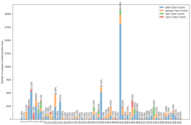
\includegraphics[width=\textwidth]{bilder/ClassCountsPerDatasetAll.png}\centering
		\caption{Class counts for labels in all datasets.}
	\end{subfigure}

	\begin{subfigure}[t]{0.90\hsize}\centering
		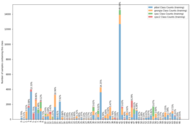
\includegraphics[width=\textwidth]{bilder/ClassCountsPerDatasetTrain.png}\centering
		\caption{Class counts for labels in the training datasets.}
	\end{subfigure}
	\label{fig:ClassCountsBar}
\end{figure}

Since we have multiple possible class labels per patient it might be interesting to see if any of the classes have a correlation to each other. For that we created \autoref{fig:ClassCountsHeatCorrelation} which shows the Pearson correlation coefficient.
%\begin{figure}[H]
%	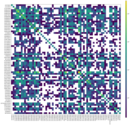
\includegraphics[width=\textwidth]{bilder/ClassOccurences.png}
%	\caption{Logarithmic Class occurrences heatmap: Given class $x$, what other classes $y$ also appear at the same patient?}
%	\label{fig:ClassCountsHeat}
%\end{figure}
\begin{figure}[H]
	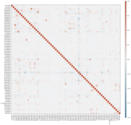
\includegraphics[width=\textwidth]{bilder/ClassOccurencesCorrelation.png}
	\caption{Pearson Class Correlation Coefficient $\rho_{X,Y}$ heatmap: Given class $x$, what other classes $y$ are likely to appear at the same patient?. $\rho_{X,Y}>0=$ positive correlation, $\rho_{X,Y}<0=$ negative correlation, $\rho_{X,Y}\approx 0$ no correlation}
	\label{fig:ClassCountsHeatCorrelation}
\end{figure}


Understanding and classifying ECG data (in real time) using an automated computer system could greatly help the likelihood of surviving an (incoming) infarction, since analysis by eye is time consuming and demands a trained medical professional. Monitoring patients at all times in the hospital could also be a great benefit. While doctors will probably still be mandatory to make the final diagnosis and prescribe medication, an automated classification system that also shows potential highly diagnostic locations in the signal could reduce analysis time by a big factor.



To address the problem of few data being publicly available, solutions different to fully supervised trained models could have a big impact on their success.

One of those more unsupervised learning domains is representation learning.

\subsection{Representation Learning/Background} \label{representation-learning}

In representation/feature learning the algorithm (neural net), tries to learn representations, often in a lower dimension, by not using the real labels directly and instead uses secondary labels extracted from the data itself. After training on these artificial labels, most layers will be used again with their weights to train on the downstream task - the task to predict the desired primary labels. As such representation learning can be split into a pretraining and training phase, which are both needed to produce a working prediction model. The strength of representation learning comes from the fact that unlabeled data is often easier to come by, but which cannot be used by fully supervised methods.

Following Yann LeCun, this is also referred to as self-supervised learning\autocite{YANNLECUNFacebookUnsupervised}, which is partly unsupervised learning since the models do not need the original labels, but there is also an supervisional aspect, where one needs to define secondary labels, related to the downstream task. 

There are many different approaches to representation learning, some train the biggest fraction of the layers using labels that can be extracted with high certainty from the data directly (Jigsaw from image \autocite{noroozi2017unsupervised}, Image Rotation \autocite{gidaris2018unsupervised}, \autocite{doersch2016unsupervised}). Others augment the data and the neural net has to calculate the same lower dimensional representation for both augmented images \autocite{chen2020simple}. 

Another way to learn representation is to predict missing or contextual information, eg. by blacking out known parts of the data and training an algorithm to fill these spots out again. The algorithm will have to find meaningful representations and thus "understand" the data in order predict the missing spots correctly. 

It is hypothesized that solving secondary tasks or predicting contextual information "are fruitful partly because the context from which we predict related values are often conditionally dependent on the same shared high-level latent information" \autocite{DBLP:journals/corr/abs-1807-03748}. That is to say by solving a secondary task and learning representations useful for that specific task, the model will be easier to train on the real problem because the necessary representations are similar to the ones already learned.

Unfortunately the methods mentioned above focus on image recognition and use knowledge not applicable to general sequential data. Also predicting high dimensional data is a very difficult task and simpler loss functions like Mean Squared Error do not work very well. Furthermore architectures like Recurrent Neural Nets that predict only one "step" into the future will likely resort to exploiting "local smoothness" - learning features that only describe the data locally but fail to infer a more global data description.

That's where methods like CPC, short for Contrastive Predictive Coding from the paper "Representation Learning using Contrastive Predictive Coding"\autocite{DBLP:journals/corr/abs-1807-03748} come into play. 

\subsection{Contrastive Predictive Coding}
\subsubsection{Overview}
\label{section:cpcindetail}
The goal of CPC is to learn data representations in a compact (latent) embedding space, which are universally useful in downstream tasks. CPC learns these representations by predicting the future not in the sequential input data, but rather its latent lower dimensional space. Due to the lower dimension, correct predictions of future latents are easier to model. Since there is no ground truth in the unknown embedding space, the architecture is trained with the help of a loss based on Noise-Contrastive Estimation, where the model has to differentiate between latents that stem from the current sample or other samples in the batch.

\begin{figure}[h]
	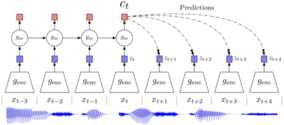
\includegraphics[width=\textwidth]{bilder/Audio-Architecture.png}
	\caption{CPC audio architecture how it is visualized in \autocite{DBLP:journals/corr/abs-1807-03748}}
	\label{cpc-architecture}
	\centering
\end{figure}

\begin{figure}[h]
	\centering
	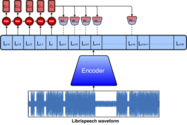
\includegraphics[width=0.8\textwidth]{bilder/CPC-correct-architecture.png}
	\caption{CPC audio architecture how it is visualized in \autocite{lai2019contrastive}}
	\label{fig:cpc-architecture-intersect}
\end{figure}

Both \autoref{cpc-architecture} and \autoref{fig:cpc-architecture-intersect} are CPC architectures, only differing in how the encoder encodes the data into latent representations. They can be used as a close reference for the following description:

First, CPC transforms the sequential data signal $x$ into multiple latent variable vectors $(z_{t-m}\ldots z_t, z_{t+1},\ldots, z_{t+k}, \ldots, z_{t+n})=g_{enc}(x)$ in an embedding space (with potentially lower dimension), using any encoder network. In \autoref{cpc-architecture} $g_{enc}$ encodes parts of the data separately, in \autoref{fig:cpc-architecture-intersect} the Encoder calculates all latents "in one go". $t$ denotes the "current" timestep, $m$ and $n$ are steps into the past and future respectively and may vary depending on chosen architecture/hyperparameters and input data.  The "past" latents $z_{t-m}\ldots z_{t}$ are fed into any recurrent network/autoregressive model (e.g. $g_{ar}$ in \autoref{cpc-architecture}), which produces a context matrix $g_{ar}(z_{t-m}, \ldots, z_{t})=(c_{t-m}, \ldots, c_{t})$, where $c_t$ is the context vector for all seen latents $z_{t-m},\ldots, z_{t}$. Since an autoregressive model is used, any number of latent vectors can be summarized into a context, which can also be sized differently from the latent vectors. The last context $c_t$ is then multiplied individually with $n$ weight matrices $W_1,\ldots, W_n$ to predict $n$ future latent vectors $\hat{z}_{t+1},\ldots, \hat{z}_{t+n}$. Multiple latents are predicted at the same time to counteract the exploitation of local smoothness and force the network to encode globally useful information into the context. In the best case scenario the context represents a meaningful description of all past latents and will be a good feature matrix for following downstream tasks. The disparity between the predicted latents $\hat{z}$ and the latents $z$, produced by the encoder network earlier, can then be used to form the loss and thus train both the encoder and autoregressive model jointly. 

To avoid a trivial encoding of e.g. an all-zero-vector for all latents, a loss based on noise contrastive estimation \autocite{pmlr-v9-gutmann10a} is used, where the network has to differentiate between positive and negative samples. Positive samples are latents that stem from $p(x_{t+k}|c_t)$ --- the same datasource that the context was calculated from. Negative samples are latents that were calculated from $p(x_{t+k})$ --- the unconditioned data distribution, independent from the current context. Negative samples can e.g. be taken from the data batch or in concrete terms another patient.



\subsubsection{Motivation} \label{sec:motivation}
As in \autoref{representation-learning} already said it is assumed that unsupervised representation learning approaches "are fruitful partly because the context from which we predict related values are often conditionally dependent on the same shared high-level latent information" \autocite{DBLP:journals/corr/abs-1807-03748}. With this motivation we want to learn features (latent representations) that maximize the mutual information between the original input and the encoded representations. Mutual information describes how much two probability density functions have in common and how much knowing one leads to knowledge about the other. "More specifically, it quantifies the "amount of information" [...] obtained about one random variable through observing the other random variable". \autocite{MutualinformationWikipedia-2021-03-25}
The equation for mutual information for two probability mass functions is given by \autoref{mutual-information}, where we arrive exactly at the papers definition in the second to last line. Here $x \in X$ are samples from the original signal and $C$ the contexts derived by $x\in X$:
\begin{equation}
	\label{mutual-information}
	\begin{aligned}
		I(X;C)&=\sum_{c\in C}\sum_{x\in X}p_{X,C}(x,c)\log\left(\frac{p_{X,C}(x,c)}{p_X(x)p_C(c)}\right)\\
		&=\sum_{c\in C}\sum_{x\in X}p_{X,C}(x,c)\log\left(\frac{p_{X,C}(x|c)p_C(c)}{p_X(x)p_C(c)}\right)\\
		&=\sum_{c, x}p(x,c)\log\left(\frac{p(x|c)}{p(x)}\right)\\
		&=\EX\log\left(\frac{p(x|c)}{p(x)}\right)
	\end{aligned}
\end{equation}
Mutual Information $I(X; C)$ could thus be described as the mean logarithmic difference between the conditional and the unconditional joint probability distributions of $X$ and $C$. If the conditional probability mass function (PMF) is similar to the unconditional PMF ($\implies X \perp C$), the difference will be close to 0. If the logarithmic difference is bigger, we know that that $X$ and $C$ are conditionally dependent, which means they have a higher Mutual Information.

As our goal, we want to find weights for our model, that \textbf{maximize the mutual information between the input signal $X$ and the calculated context $C$}.

\subsubsection{Math in detail}
To reach our goal, we define the probability that given a context $c_t$ and a set of samples $X$, a specific sample $x_i \in X$ was drawn from the conditional distribution $p(x_{t+k}|c_t)$, rather than from the unconditional distribution $p(x_{t+k})$.
This probability is given by \autoref{eq:pdi} with $[d = i]$ being the indicator that sample $x_i$ is the "positive" sample \autocite[4]{DBLP:journals/corr/abs-1807-03748}:
\begin{equation}
	\begin{aligned}
		p(d=i|X, c_t) &= \frac{p(x_i|c_t)\prod_{l\neq i}p(x_l)}{\sum_{j=1}^{N}p(x_j|c_t)\prod_{l\neq j}p(x_l)} \label{eq:pdi}\\
		&=\frac{p(x_i|c_t)\left(\frac{1}{p(x_i)}\prod_{l=1}^{N}p(x_l)\right)}{\sum_{j=1}^{N}p(x_j|c_t)\left(\frac{1}{p(x_j)}\prod_{l=1}^{N}p(x_l)\right)}\\
		&=\frac{\frac{p(x_i|c_t)}{p(x_i)}}{\sum_{j=1}^{N}\frac{p(x_j|c_t)}{p(x_j)}}\\ 
	\end{aligned}%%&=\frac{p(x_i|c_t)\frac{1}{p(x_i)}}{\sum_{j=1}^{N}p(x_j|c_t)\frac{1}{p(x_j)}}\\
\end{equation}


In \autoref{eq:pdi} the numerator $p(x_i|c_t)\prod_{l\neq i}p(x_l)$ is the probability that $x_i$ was drawn from $p(x_{t+k}|c_t)$, while all other $x_{j}\in X, j\neq i$ were drawn from $p(x_{t+k})$. This gets normalized by $\sum_{j=1}^{N}p(x_j|c_t)\prod_{l\neq j}p(x_l)$, the sum of all probabilities where $x_j$ was drawn from $p(x_{t+k}|c_t)$ instead of $x_i$. Note that $p(x_i|c_t)\prod_{l\neq i}p(x_l)$ is also included in the sum, thus $p(d=i|X, c_t) \in [0,1]$.

The goal of the loss function will be to maximize this probability over all possible combinations between each sample and the corresponding context. Which means the model will need to distinguish between positive and negative samples, given a context. Knowing that the mutual information means: given $C$, how much do we know about $X$, it becomes clear that a model that maximized the mutual information between the original signal and its context, will have an easier "job" to distinguish between real and wrong sample.

The categorical cross entropy loss is a commonly used loss function for training on class probability scores for $N$ classes:
$\sum_{i=1}^{N}y_ilog(\hat{y}_i)$ --- where $y_i$ is the ground truth - and $\hat{y}_i$ is the model prediction.

Combining both the cross entropy loss with \autoref{eq:pdi}, we arrive at the following loss function:
\begin{equation}
	\begin{aligned}
		\mathcal{L_N} &=-\underset{x_i\in X}{\EX}\log\left[\frac{\frac{p(x_i|c_t)}{p(x_i)}}{\underset{x_j\in X}{\sum}\frac{p(x_j|c_t)}{p(x_j)}}\right]
	\end{aligned}
\end{equation}
However, since we cannot evaluate $\frac{p(x_{t+k}|c_t)}{p(x_{t+k})}$ directly, we need a function $f$ s.t. $f_k(x_{t+k}, c_t) \propto \frac{p(x_{t+k}|c_t)}{p(x_{t+k})}$,  ($f$ needs to only be proportional to the optimal value and is not restricted to lay in the interval $[0,1]$). In the paper $f_k(x_{t+k}, c_t) := \exp \left( z_{t+k}^T W_kc_t\right)$ is used to form a simple log-bilinear model. $W_kc_t$ is the models prediction for latent $z_{t+k}$, the dot product between the prediction and the ground truth expresses their similarity, because the dot product between two vectors implies whether they point in the same/opposing/orthogonal direction. This log-bilinear model is also used in the well-known word2vec model in natural language processing \autocite{mikolov2013efficient}.

We thus finally arrive at the InfoNCE loss function from the paper (which can also be described as the logarithmic Softmax over vector similarities): 
\begin{equation}
	\begin{aligned}
		\mathcal{L_N}&=-\underset{X}{\EX}\log\left[\frac{f_k(x_{t+k}, c_t)}{\underset{x_j\in X}{\sum}f_k(x_{j}, c_t)}\right]\\
		&:=-\underset{X}{\EX}\log\left[\frac{\exp \left( z_{t+k}^T W_kc_t\right)}{\underset{x_j\in X}{\sum}\exp \left( z_{j}^T W_kc_t\right)}\right]
	\end{aligned}
\end{equation}

The prove from the original paper, that this loss is indeed maximizing the mutual information between $c_t$ and $x_{t+k}$, is given here with additional steps for easier following (\autoref{eqn:cpc-prove}). For $f_k(x_{j}, c_t)$ it uses the optimal value $\frac{p(x_{t+k}|c_t)}{p( x_{t+k})}$ instead of $\exp \left( z_{t+k}^T W_kc_t\right)$:
\begin{align} \label{eqn:cpc-prove}
	\intertext{Given a set $X$ split into one positive sample $x_{t+k}$ and $N-1$ negative samples $X_{neg}$.}
	\mathcal{L}^{opt}_N &=-\underset{X}{\EX}\log\left[\frac{\frac{p( x_{t+k}|c_t)}{p( x_{t+k})}}{\underset{x_j\in X}{\sum}\frac{p(x_j|c_t)}{p(x_j)}}\right]\\	
	&=-\underset{X}{\EX}\log\left[\frac{\frac{p( x_{t+k}|c_t)}{p( x_{t+k})}}{\frac{p( x_{t+k}|c_t)}{p( x_{t+k})} + \underset{x_j\in X_{neg}}{\sum}\frac{p(x_j|c_t)}{p(x_j)}}\right]\\
	&=\underset{X}{\EX}\log\left[\frac{\frac{p( x_{t+k}|c_t)}{p( x_{t+k})} + \underset{x_j\in X_{neg}}{\sum}\frac{p(x_j|c_t)}{p(x_j)}}{\frac{p( x_{t+k}|c_t)}{p( x_{t+k})}}\right]\\
	&=\underset{X}{\EX}\log\left[\frac{p( x_{t+k})}{p( x_{t+k}|c_t)} \cdot \left(\frac{p( x_{t+k}|c_t)}{p( x_{t+k})} + \underset{x_j\in X_{neg}}{\sum}\frac{p(x_j|c_t)}{p(x_j)}\right)\right]\\
	&=\underset{X}{\EX}\log\left[1 + \frac{p( x_{t+k})}{p( x_{t+k}|c_t)}\underset{x_j\in X_{neg}}{\sum}\frac{p(x_j|c_t)}{p(x_j)}\right]\\
	&=\underset{X}{\EX}\log\left[1 + \frac{p( x_{t+k})}{p( x_{t+k}|c_t)}(N-1)\underset{x_j\in X_{neg}}{\sum}\frac{1}{N-1}\frac{p(x_j|c_t)}{p(x_j)}\right]\\
	\intertext{Assuming all $N-1$ negative samples have approximately the same probability:}
	&=\underset{X}{\EX}\log\left[1 + \frac{p( x_{t+k})}{p( x_{t+k}|c_t)}(N-1)\underset{x_j\in X_{neg}}{\EX}\frac{p(x_j|c_t)}{p(x_j)}\right]\\
	&\approx\underset{X}{\EX}\log\left[1 + \frac{p( x_{t+k})}{p( x_{t+k}|c_t)}(N-1)\right], \text{Assuming $c_t$, $x_j$ are (nearly) independent} \\
	&=\underset{X}{\EX}\log\left[\frac{p( x_{t+k})}{p( x_{t+k}|c_t)}N + 1 - \frac{p( x_{t+k})}{p( x_{t+k}|c_t)}\right]\\
	&\geq\underset{X}{\EX}\log\left[\frac{p( x_{t+k})}{p( x_{t+k}|c_t)}N\right], \text{Assuming $p( x_{t+k}) \leq p( x_{t+k}|c_t)$}\\
	&=-\underset{X}{\EX}\log\left[\frac{p( x_{t+k}|c_t)}{p( x_{t+k})}\right]+\log(N)\\
	&=-I(x_{t+k}, c_t) + \log(N)
\end{align}
Therefore $-I(x_{t+k}, c_t) \geq \log(N) - \mathcal{L}^{opt}_N$, which is also true for loss functions greater than $\mathcal{L}^{opt}_N$ (with non optimal $f \propto \frac{p(x_i|c_t)}{p(x_i)})$. \enquote{Equation (15) quickly becomes more accurate as $N$ increases. At the same time $\log(N)-\mathcal{L}_N$ also increases, so it's useful to use large values of $N$} \autocite{DBLP:journals/corr/abs-1807-03748}.

\subsubsection{Algorithm}
The original CPC Loss formulation can be seen in \autoref{fig:cpcorigloss}.
\begin{tcolorbox}
	\begin{figure}[H]
		\centering
		\caption{"Given a set $X = {x_1, \ldots, x_N }$ of $N$ random samples containing one positive sample from $p(x_{t+k}|c_t)$ and $N - 1$ negative samples from [...] $p(x_{t+k})$, we optimize":}
		\begin{equation}
			\begin{aligned}
				L_N &=-\underset{X}{\EX}\log\left[\frac{f_k(x_{t+k}, c_t)}{\underset{x_j\in X}{\sum}f_k(x_{j}, c_t)}\right]\\
				&:=-\underset{X}{\EX}\log\left[\frac{\exp \left( z_{t+k}^T W_kc_t\right)}{\underset{x_j\in X}{\sum}\exp \left(z_{j}^TW_kc_t\right)}\right] \nonumber
			\end{aligned}
		\end{equation}	
		\subcaption{InfoNCE Loss from \autocite{DBLP:journals/corr/abs-1807-03748}}
		\label{fig:cpcorigloss}
	\end{figure}
\end{tcolorbox}

However we think that this formulation can be misunderstood once it has to be implemented and hence give a mathematical formulation more along the lines of the second paper \autocite{cpcdataefficient}. Note that this version uses every sample $x_i \in X$ once as a positive sample: \autoref{algorithm:cpc-algo}
\RestyleAlgo{boxruled}
\begin{algorithm}[H]
	\caption{InfoNCE Loss calculation}
	\KwData{A set of $N$ \emph{full} data-samples $X=(x_1, \ldots, x_N)$. }
	\tcc{\mycommfont{$X$ can e.g. be a set/batch of patients' ECG records with size $ N \times \mathit{channels} \times \mathit{datalength}$}}
	\KwIn{An index $t\in \mathbb{N}$.}
	\tcc{\mycommfont{$t$ marks the "present" timestep and splits data into "past" and "future". }}
	\KwIn{The encoder network $g_{enc}(x_i|\theta)\mapsto z_i=(z_{i, 1}, \ldots, z_{i, t}, z_{i, t+1}, \ldots, z_{i, t+k})$}
	\tcc{\mycommfont{$z_i$ is a set of $t+k$ latent vectors, representing consecutive timesteps of the input data in a lower dimension. How many get produced is dependent on the encoder network and data samples $x \in X$}}
	\KwIn{The context network $g_{ar}((z_{i, 1}, z_{i, 2}, \ldots, z_{i, t})|\psi) \mapsto c_{i,t}$}
	\tcc{\mycommfont{$c_{i,t}$ is the context vector for a set of $t$ latent vectors, for data-sample $x_i$}}
	\KwIn{A set of $n$ weight matrices $\{W_1 \ldots W_n$\}}
	\tcc{\mycommfont{The weight matrices are used to calculate a set of $n$ latent vectors} $\hat{z}_{i}=(\hat{z}_{i, t+1}, \ldots, \hat{z}_{i, t+n}) := (W_1c_{i, t}, W_2c_{i, t}, \ldots, W_nc_{i, t})$}
	\KwResult{
	\begin{flushleft}		
		\[\mathit{Loss}_i := -\frac{1}{k}\sum_{k=1}^{n}\log\left[\frac{\exp(\hat{z}_{i, t+k}^Tz_{i, t+k})}{\exp(\hat{z}_{i, t+k}^Tz_{i, t+k})+\underset{{(j,l)\in \{(j,l)|j\neq i \land l \leq |z_i|\}}}{\sum \exp(\hat{z}_{i, t+k}^Tz_{j, l})}}\right]\]
		\tcc{\mycommfont{$\mathit{Loss}_i$ is the scalar loss value for a single positive data-sample $x_i$. This is close to the papers definition.}}
		
		\[\mathit{Loss} := \frac{1}{N}\sum_{i=1}^{N}\mathit{Loss}_i=\]
		\[=-\frac{1}{kN}\sum_{i=1}^{N}\sum_{k=1}^{k}\log\left[\frac{\exp(\hat{z}_{i, t+k}^Tz_{i, t+k})}{\exp(\hat{z}_{i, t+k}^Tz_{i, t+k})+\sum_{(j,l)\in \{(j,l)|j\neq i \land l \leq |z_i|\}}\exp(\hat{z}_{i, t+k}^Tz_{j, l})}\right]\]
		\tcc{\mycommfont{$\mathit{Loss}$ is the scalar loss value where each data-samples $x_i\in X$ is the positive sample once.}}
	\end{flushleft}}
	\label{algorithm:cpc-algo}
\end{algorithm}
Note that the set of negative latent samples $A:=\{(j,l)|j\neq i \land l \leq |z_i|\}$ can be replaced by e.g. $A_1\subset\{(j,l)|j\neq i \land l \leq |z_i|\} \leftrightarrow A_1 \textit{ is a random subset of }A$, if there are too many negative samples for the hardware to handle, or by e.g.
$A_2:=\{(j,l)|j\neq i \land l = t+k\}\leftrightarrow A_2 \textit{ is only using negative examples that share the same timestep as }z_{i, t+k}$, to provide samples that might be more similar to the positive one.

Furthermore we provide an algorithm in Python pseudo code from our understanding, to further explain the loss function and clear up potential confusion. \autoref{algo:cpcslow} shows this pseudo code for a naive implementation of the formula we provided in \autoref{algorithm:cpc-algo} (with negative samples that stem from other batches but the same timestep).
\begin{minipage}{\linewidth}
\begin{lstlisting}[language=Python, caption=Naive CPC Loss Pseudo Code, label=algo:cpcslow]
def cpc_loss_naive(X:Tensor, W:List[Tensor], enc:nn.Module, rnn:nn.Module):
	batch, channels, data_length = X.shape #eg. (64 x 12 x 4500)
	#Encode data into latents:
	latent_matrix = enc(X)
	batch, timesteps, latent_size = latent_matrix.shape #eg. (64 x 27 x 128)
	#Calculate context from latents:
	context_matrix = rnn(latent_matrix)
	batch, timesteps, context_size = context_matrix.shape #eg. (64 x 27 x 256)
	#Select current timestep (here last possible):
	n=len(W)
	current_timestep = timesteps-n-1
	last_context_vector = context_matrix[:, current_timestep, :]
	#output shape: (64 x 256)
	loss = 0.        
	for i in range(batch):
		loss_i = 0.    
		for k in range(n):
			#Predict latent for specific timestep k from current context:
			latent_vector_pred_i = last_context_vector[i] @ W[k]
			#Select latent vector for batch i at correct timestep:
			latent_vector_i = latent_matrix[i, current_timestep+k+1, :] 
			#calculate similiarity with dot product:
			sim = latent_vector_pred_i @ latent_vector_i #scalar
			#calculate exp(sim) for softmax
			p_xi_ct = exp(sim) 
			nominator = p_xi_ct
			denominator = 0.
			for j in range(batch): #replace j with j, l for different sampling
				latent_vector_j = latent_matrix[j, current_timestep+k+1, :] 
				#Calculate dot product to measure similarity:
				sim = latent_vector_pred_i @ latent_vector_j #scalar
				#Calculate exp(sim) for softmax
				p_xj_ct = exp(sim) 
				denominator += p_xj_ct
			#take log for log softmax
			loss_i += log(nominator/denominator)
		loss += -loss_i/n
	return loss / batch
\end{lstlisting}

\end{minipage}

\begin{minipage}{\linewidth}
	\begin{lstlisting}[language=Python, caption=Optimized CPC Loss Pseudo Code. Uses CrossEntropyLoss from Pytorch, label=algo:cpcfast]
def cpc_loss_fast(X:Tensor, W:List[nn.Module], enc:nn.Module, rnn:nn.Module):
	
	batch, channels, data_length = X.shape #eg. (64 x 12 x 4500)
	
	latent_matrix = enc(X)
	batch, timesteps, latent_size = latent_matrix.shape #eg. (64 x 27 x 128)
	
	context_matrix = rnn(latent_matrix)
	batch, timesteps, context_size = context_matrix.shape #eg. (64 x 27 x 256)
	
	timesteps_out = len(W) #eg. 12
	current_timestep = timesteps-timesteps_out
	last_context_vector = context_matrix[:, current_timestep-1, :] #shape: (64 x 256)
	loss = 0.
	accuracy = 0.
	for k in range(timesteps_out):
		#predict latents for timestep k and all items in batch:
		pred_latent = W[k](last_context_vector) #shape: (64 x 128)
		#calculate similarity between all encoded latents against pred_latent:
		sim = latent_matrix @ pred_latent.T #shape eg.: (64 x 27 x 64)
		#reshape result for easier/efficient indexing:
		sim_r = sim.reshape(timesteps*batch, batch).T #shape eg.: (64, 1728)
		#Select the indices where pred_{i,k}==latent_{i,k}
		labels = torch.arange(batch) + batch*(current_timestep + k)
		#pytorch: crossentropyloss = LogSoftmax + NLL_Loss
		loss += crossentropyloss(sim_r, labels)
		#Count how often the max softmax value is at the correct idx
		accuracy += (sim_r.max(dim=-1).indices == labels).sum()
	
	loss = loss / (timesteps_out*batch)
	accuracy = accuracy / (timesteps_out*batch)  # * pred_latent.shape[0]
	return accuracy, loss, hidden
	\end{lstlisting}

\end{minipage}